\section{Criação do canal no ThingSpeak}

Para gerar o gráfico, acessamos o site do \href{https://thingspeak.mathworks.com/}{ThingSpeak}. É necessário criar uma conta no site, então apertamos em "Get Started For Free". Só é possível criar uma conta com um email institucional ou de uma empresa.

\begin{figure}[H]
    \centering
    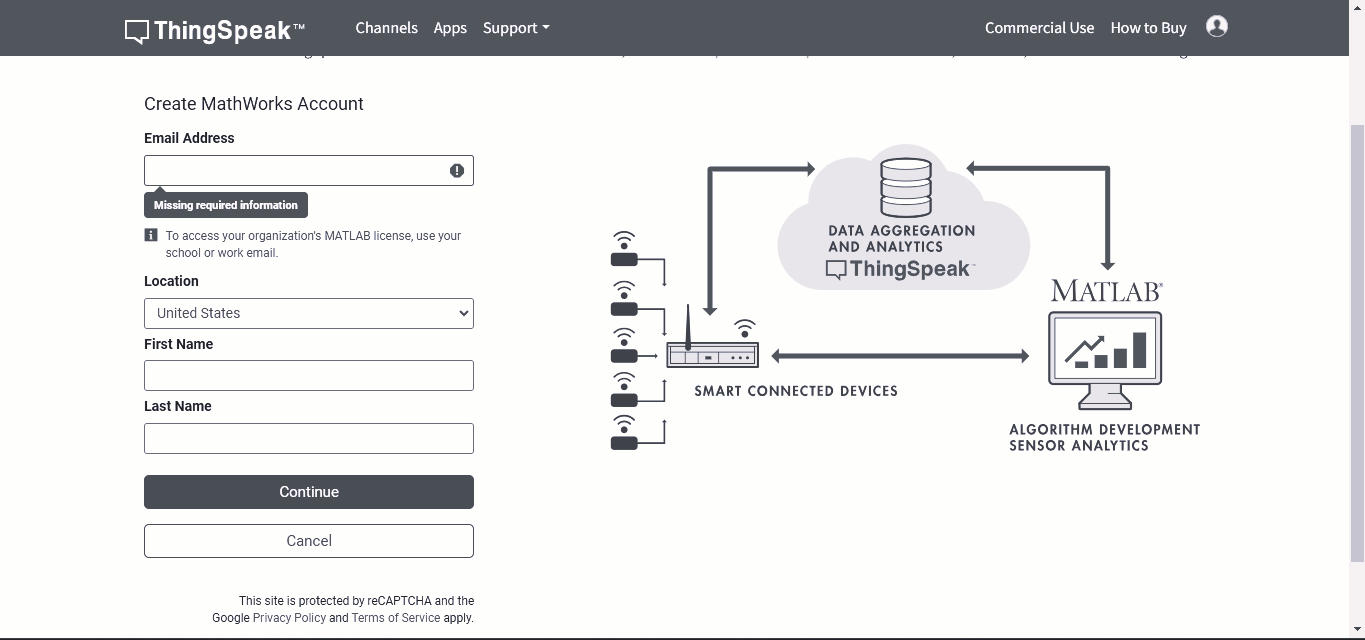
\includegraphics[width=0.5\linewidth]{img/Thinkspeak.png}
    \caption{Tela de cadastro do ThingSpeak.}
    \label{fig:thingspeak-sign-up}
\end{figure}

Com a conta criada, acessamos a aba Channel e criamos um novo canal. Preenchendo o nome e os campos do canal.

\begin{figure}[H]
    \centering
    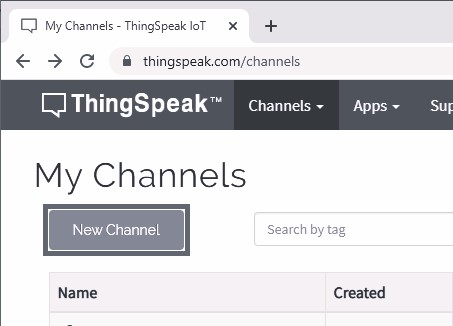
\includegraphics[width=0.5\linewidth]{img/ThingSpeak-New-Channel.jpg}
    \caption{Botão para criar canais no ThingSpeak.}
    \label{fig:thingspeak-create-channel}
\end{figure}

Com o canal criado, clicamos no símbolo de um lápis para editá-lo. Podemos preencher os campos, mas o mais importante é acessar a aba "API Keys" e copiar a chave de API de escrita, para publicarmos os dados que vamos descobrir com o potenciômetro.

\begin{figure}[H]
    \centering
    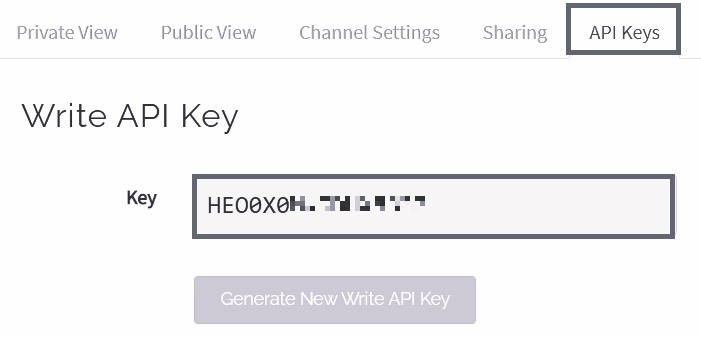
\includegraphics[width=0.5\linewidth]{img/Thingspeak-Write-API-key.jpg}
    \caption{Chave de escrita do ThingSpeak.}
    \label{fig:thingspeak-api-key}
\end{figure}